The framework test was done with the model indicated in the assignemtns. We decided to create three different datasets: training, validation and test. The first is used for the training procedure, the second to check improvements of the training results and to check for possible overfitting, the third to check the final results. \\
The test was performed with the model described below, using the compute history and real-time graphic visualization functionality.
\begin{minted}{Python}
model = nn.Sequential(
	nn.Dense(2, 25, F.ReLU()),
	nn.Dense(25, 25, F.ReLU()),
	nn.Dense(25, 25, F.ReLU()),
	nn.Dense(25, 2, F.Sigmoid())
)  
\end{minted}
The model consists in a three-layer network with ReLU activation functions in the hidden layers and a Sigmoid as output function. Sigmoid function fits perfectly with a 2-classes classification problem because the result is within [0 - 1]. 

\begin{comment}
The 'Dynamic results on validation dataset' picture represents the performance of the network after 30 epochs on validation dataset. The green area represents the zone where the network predicts 1, the red area is where it predicts 0. Green dots are samples 1 that are correctly predicted by the net, red dots are the correct 0 samples, blue ones are mispredicted samples.
\begin{figure}[H]
	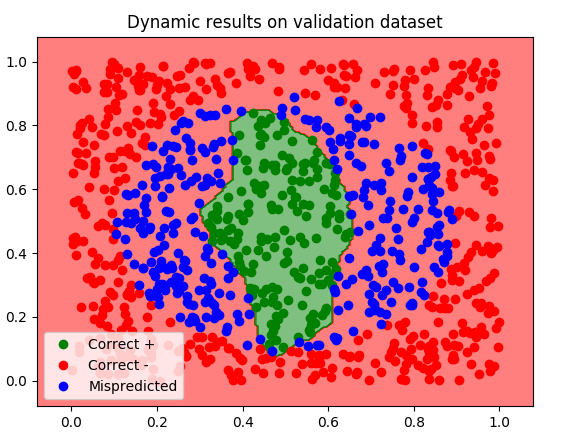
\includegraphics[width=8cm]{Images/30epochs.png}
	\centering
\end{figure}


This figure shows the network trend in terms of loss and accuracy, both for training and validation dataset. The graph shows a divergence in the losses around the 2000th epoch; this is a first sign of overfitting.
\begin{figure}[H]
	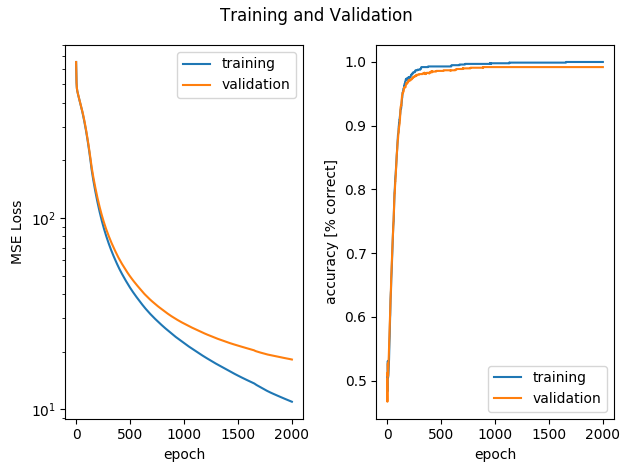
\includegraphics[width=8cm]{Images/LossAccFinal.png}
	\centering
\end{figure}

The last image shows the network performances on the test dataset. As written in the caption, it perforates 99.1\% on the test, in fact only the 9 blue dots on a dataset of 1000 samples are labeled incorrectly.

\begin{figure}[H]
	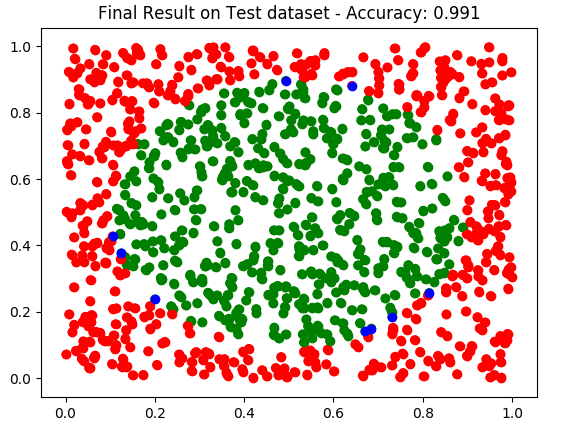
\includegraphics[width=8cm]{Images/FinalTestAccuracy.png}
	\centering
\end{figure}

\end{comment}

\begin{minipage}{0.45\textwidth} 
	The 'Dynamic results on validation dataset' picture represents the performance of the network after 30 epochs on validation dataset. The green area represents the zone where the network predicts 1, the red area is where it predicts 0. Green dots are samples 1 that are correctly predicted by the net, red dots are the correct 0 samples, blue ones are mispredicted samples.
\end{minipage}
\begin{minipage}{0.5\textwidth} \raggedleft 
	\begin{figure}[H]
		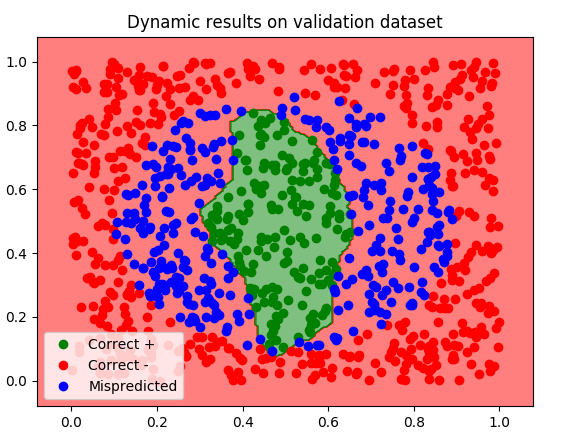
\includegraphics[width=0.9\textwidth]{Images/30epochs.png}
		\centering
		\caption{dlds}
		\centering
	\end{figure}
\end{minipage}


\vspace{-0.5cm}
\begin{minipage}{0.45\textwidth} 
	This figure shows the network trend in terms of loss and accuracy, both for training and validation dataset. The graph shows a divergence in the losses around the 2000th epoch; this is a first sign of overfitting.
\end{minipage}
\begin{minipage}{0.5\textwidth} \raggedleft 
	\begin{figure}[H]
		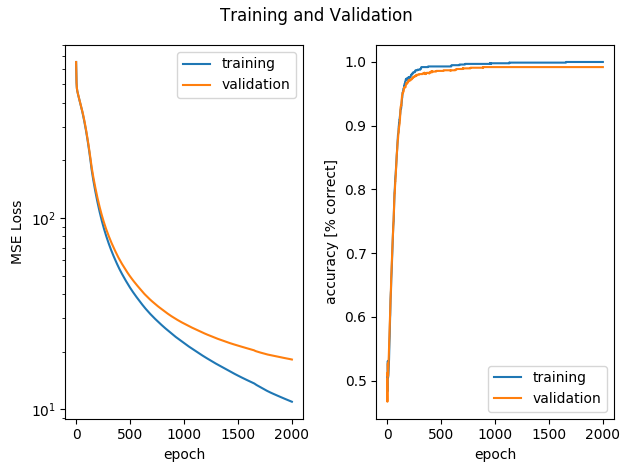
\includegraphics[width=0.9\textwidth]{Images/LossAccFinal.png}
		\centering
		\caption{dlds}
		\centering
	\end{figure}
\end{minipage}

\vspace{-1cm}
\begin{minipage}{0.45\textwidth} 
	The last image shows the network performances on the test dataset. As written in the caption, it perforates 99.1\% on the test, in fact only the 9 blue dots on a dataset of 1000 samples are labeled incorrectly.
\end{minipage}
\begin{minipage}{0.5\textwidth} \raggedleft 
	\begin{figure}[H]
		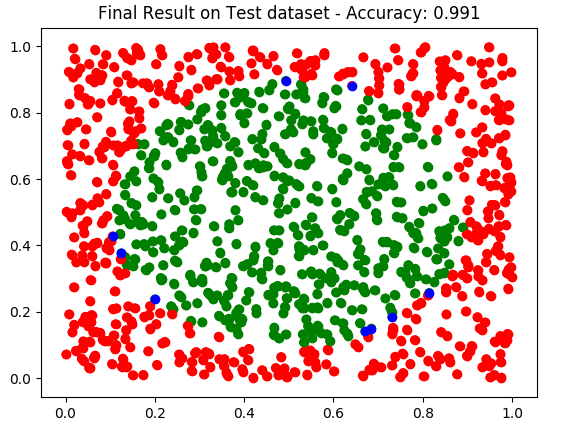
\includegraphics[width=0.9\textwidth]{Images/FinalTestAccuracy.png}
		\centering
		\caption{dlds}
		\centering
	\end{figure}
\end{minipage}

